\documentclass[english,10pt,c]{beamer}

\usepackage{etex}
\usepackage[T1]{fontenc}
\usepackage{babel}
\usepackage{lipsum}
\usefonttheme{structuresmallcapsserif}
\usefonttheme{serif}
\usepackage[utf8]{inputenc}
%\usepackage{natbib}
\usepackage{colortbl}
\usepackage{tipa}   %for IPA
\usepackage{amstext} 
\usepackage{amsmath}
\usepackage{amssymb}
\usepackage{listings} %for displaying code
%\usepackage{enumitem}
\usepackage{graphicx}
\usepackage{qtree}    %for trees
\usepackage{tikz}
\usepackage{tikz-qtree}
\usetikzlibrary{shapes,positioning}
\usepackage{multicol}
\usepackage{multirow}
\usepackage{stmaryrd} 
\usepackage{arydshln} 
\usepackage{ulem}
\usepackage{hyperref}
\definecolor{links}{HTML}{2A1B81}
\hypersetup{colorlinks,linkcolor=,urlcolor=links}
\usepackage{pifont} %for symbols
%\usepackage{dsfont}	%for more symbols
\usepackage{gb4e} 	%for linguistic examples and glosses

\newcommand{\vs}{\vspace{11pt}}		%makes a vertical skip of 12pts
\newcommand{\underscore}{\underline{\hspace{0.5cm}}}		%0.5 cm long underline
%\let\eachwordtwo=\sc

\AtBeginSection[]
{
  \begin{frame}
    \frametitle{Table of Contents}
    \tableofcontents[currentsection]
  \end{frame}
}

%\usetheme{CambridgeUS}

%    \setbeamertemplate{frametitle}
%      {\begin{centering}\smallskip
%       \insertframetitle\par
%       \smallskip\end{centering}}
%    \setbeamertemplate{itemize item}{$\bullet$}
%    \setbeamertemplate{navigation symbols}{}
%    \setbeamertemplate{footline}[text line]{%
%        \hfill\strut{%
%            \scriptsize\sf\color{black!60}%
%           % \quad\insertframenumber
%        }%
%        \hfill
%    }


\useoutertheme{smoothbars}
 \setbeamertemplate{itemize item}{$\bullet$}
\setbeamertemplate{footline}[frame number]
\setbeamertemplate{frametitle}{
\begin{centering}
\insertframetitle
\par
\end{centering}
} 

\definecolor{Gray}{gray}{0.9}
\definecolor{lightblue}{HTML}{81BEF7}
    % Define some colors:
    \definecolor{DarkFern}{HTML}{407428}
    \definecolor{DarkCharcoal}{HTML}{4D4944}
    \colorlet{Fern}{DarkFern!85!white}
    \colorlet{Charcoal}{DarkCharcoal!85!white}
    \colorlet{LightCharcoal}{Charcoal!50!white}
    \colorlet{AlertColor}{orange!80!black}
    \colorlet{DarkRed}{red!70!black}
    \colorlet{DarkBlue}{blue!70!black}
    \colorlet{DarkGreen}{green!70!black}
    % Use the colors:
    \setbeamercolor{title}{fg=Fern}
    \setbeamercolor{frametitle}{fg=Fern}
    \setbeamercolor{normal text}{fg=Charcoal}
    \setbeamercolor{block title}{fg=black,bg=Fern!25!white}
    \setbeamercolor{block body}{fg=black,bg=Fern!25!white}
    \setbeamercolor{alerted text}{fg=AlertColor}
    \setbeamercolor{itemize item}{fg=Charcoal}

\lstset{language=TeX,  
basicstyle=\ttfamily\color{black}\small, breaklines=true,
keywordstyle=\bfseries\color{green!40!black},
  commentstyle=\itshape\color{purple!40!black},
  identifierstyle=\color{blue},
  stringstyle=\color{orange},}

\title[] % (optional, only for long titles)
{\LaTeX Workshop}
\subtitle{}
\author[Mai Ha Vu] % (optional, for multiple authors)
{Mai Ha Vu}
\institute{University of Delaware}
\date{February 10, 2016} % (optional)

\begin{document}



%\title{LaTeX Workshop}	%title of the document
%\author{Mai Ha Vu}		%author of the document
%\date{November 3, 2013}		%date. comment out if you want current date.


\maketitle		%prints the title

\section{Latex Review}
\begin{frame}
\frametitle{Getting started}

\begin{enumerate}
\item \LaTeX distribution
\begin{itemize}
\item \href{http://www.miktex.org/download}{Windows}
\item \href{https://www.tug.org/mactex/mactex-download.html}{Max}
\item \href{https://www.tug.org/texlive/quickinstall.html}{Linux}
\end{itemize}
\item \LaTeX editor. My favorite is TexStudio.
\item Open a sample \LaTeX document in your editor, and compile it. You can find sample documents \href{http://udel.edu/~maiha/latex.html}{on my website}.
\end{enumerate}
\end{frame}

\begin{frame}[fragile]
\frametitle{Basic Structure of LaTeX documents}

\begin{enumerate}
\item Declare type of document
\begin{lstlisting}  
\documentclass[english,10pt,c]{article}
\end{lstlisting}
\item List packages to use
\begin{lstlisting}  
\usepackage{tipa}
\end{lstlisting}
\item Define macros and commands
\begin{lstlisting}
\newcommand{\vs}{\vspace{11pt}}
\end{lstlisting}
\item Begin document
\begin{lstlisting}
\begin{document}
\end{lstlisting}
\item Write things
\item End document
\begin{lstlisting}
\end{document}
\end{lstlisting}
\end{enumerate}

\end{frame}


\begin{frame}[fragile]
\frametitle{Mistakes to look out for}

\begin{itemize}
\item Commands are introduced with backslash, then add specifics in \{curly brackets\}. Optional options are in [square brackets].
\item Watch out for special symbols such as \$, \%, \{\}. You have to introduce them with backslash. 

\begin{lstlisting}
\$, \%, \{\}
\end{lstlisting}
\item Some commands only work in mathmode (.e.g $ \rightarrow $). To enter mathmode, put command between \$dollarsigns\$.

\begin{lstlisting}
$ \rightarrow $
\end{lstlisting}
\item You can comment out lines with \%
\end{itemize}
\end{frame}

\begin{frame}[fragile]
\frametitle{Basic operations}

\begin{itemize}
\item Sections 
\begin{lstlisting}
\section{Section}
\section*{Section without numbering}
\subsection{Subsection}
\subsubsection{Subsubsection}
\end{lstlisting}
\item \textbf{bold}, \textit{italics}, \underline{underlined}, \emph{emphasis}
\begin{lstlisting}
\textbf{bold}, \textit{italics}, \underline{underlined}, \emph{emphasis}
\end{lstlisting}


\end{itemize}
\end{frame}

\begin{frame}[fragile]
\frametitle{Basic operations}

\begin{enumerate}
\item List things
\begin{lstlisting}
\begin{itemize}
\item Items with bullets
\end{itemize}
\end{lstlisting}
\item Enumerate things
\begin{lstlisting}
\begin{enumerate}
\item Enumerated items
\end{enumerate}
\end{lstlisting}
\item Linguistic examples with glosses
\begin{lstlisting}
\begin{exe}
\ex[] {\gll Senki nem akar olvasni. \\
	Nobody NEG wants read.INF \\
	\trans `Nobody wants to read.'}
\end{exe}
\end{lstlisting}
\end{enumerate}

\end{frame}

\begin{frame}[fragile]
\frametitle{Basic operations}

\begin{lstlisting}
\begin{tabular}{l | c | r}
Here & is & a \\ \hline 
table & for & you! \\
\end{tabular}
\end{lstlisting}

\begin{tabular}{l | c | r}
Here & is & a \\ \hline 
table & for & you! \\
\end{tabular}
 


\end{frame}

\begin{frame}[fragile]
\frametitle{Linguistic Operations}

\begin{itemize}
\item \textipa{[AI pi eI ""t\super h\*r\ae ns"k\super h\*rIpS\s{n}z]}

\begin{lstlisting}
 \textipa{[AI pi eI ""t\super h\*r\ae ns"k\super h\*rIpS\s{n}z]}
\end{lstlisting}
\item \ 

\begin{columns} 
\column{0.2\textwidth}
	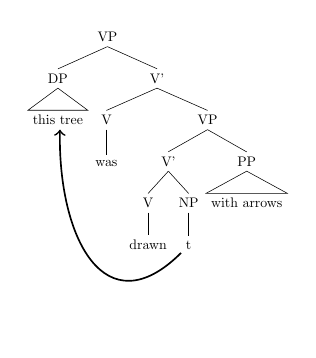
\begin{tikzpicture} [scale = 0.5]
	\Tree [.VP [.DP \edge[roof];\node(2){this tree}; ] [.V' [.V was ] [.VP [.V'  [.V drawn ] [.NP \node(1){t};  ] ] [.PP \edge[roof]; {with arrows} ] ]  ] ]
	
	\draw [semithick, ->] (1) .. controls +(south west:3) and +(south:3) .. (2);
\end{tikzpicture}
\column{0.7\textwidth}

\begin{lstlisting}
\begin{tikzpicture} [scale = 0.5]
\Tree [.VP [.DP \edge[roof];\node(2){this tree}; ] [.V' [.V was ] [.VP [.V'  [.V drawn ] [.NP \node(1){t};]] [.PP \edge[roof];{with arrows}]]]]

\draw [semithick, ->] (1) .. controls +(south west:3) and +(south:3) .. (2);
\end{tikzpicture}
\end{lstlisting}
\end{columns}
\end{itemize}
\end{frame}

\section{Beamer: Presentations and Posters}

\begin{frame}[fragile]
\frametitle{Presentations and Posters}

\begin{itemize}
\item Posters are just one slide in a presentation
\item Declare documentclass with beamer
\begin{lstlisting}
\documentclass[english,10pt,c]{beamer}
\end{lstlisting}
\item Preambles can be the same (but some packages might not be compatible with beamer!)
\item Set the style and the colors (can find a combination of all preset ones \href{https://www.hartwork.org/beamer-theme-matrix/}{here})
\begin{lstlisting}
\usetheme{Warsaw}
\usecolortheme{beaver}
\end{lstlisting}
\item Set title
\begin{lstlisting}
\title[] {\LaTeX Workshop}
\subtitle{}
\author {Mai Ha Vu}
\institute{University of Delaware}
\date{February 10, 2016} 
\end{lstlisting}
\end{itemize}
\end{frame}

\begin{frame}[containsverbatim]
\frametitle{A typical frame}

\begin{lstlisting}
\begin{frame}
\frametitle{Some Title for your Frame}

\begin{itemize}
\item Your
\item Bullet
\item Points
\end{itemize}


\includegraphics[scale=0.3]{placeholder}

\end{frame}

\end{lstlisting}

\end{frame}

\begin{frame}
\frametitle{Some Title for your Frame}

\begin{itemize}
\item Your
\item Bullet
\item Points
\end{itemize}


\includegraphics[scale=0.3]{placeholder}

\end{frame}

\begin{frame}
\frametitle{Some Title}

 \begin{columns}[t]
      \begin{column}{0.3\textwidth}
Column 1
      \end{column}
      \begin{column}{0.3\textwidth}
 Column 2
      \end{column}
      \begin{column}{0.3\textwidth}
  Column 3
       \end{column}
   \end{columns}

\end{frame}

\begin{frame}[containsverbatim]
\frametitle{Columns in the frame}

\begin{lstlisting}
\begin{frame}
\frametitle{Some Title}

\begin{columns}[t]
\begin{column}{0.3\textwidth}
	Column 1
\end{column}

\begin{column}{0.3\textwidth}
	Column 2
\end{column}

\begin{column}{0.3\textwidth}
 	Column 3
\end{column}
\end{columns}

\end{frame}
\end{lstlisting}
\end{frame}

\begin{frame}[fragile]
\frametitle{Posters}

\begin{lstlisting}
\documentclass[final]{beamer}

\usepackage[orientation=portrait, size=a0, scale=1.4]{beamerposter} % Use the beamerposter package for laying out the poster

\usetheme{confposter} % Use the confposter theme supplied with this template
\end{lstlisting}

\begin{itemize}
\item Put \emph{beamerthemeconfposter.sty} in the same folder as your poster. I haven't figured out yet how to make my \LaTeX editor know where to pull files from when needed.
\end{itemize}
\end{frame}


\begin{frame}[fragile]
\frametitle{Setting up poster size}

\begin{lstlisting}

\newlength{\sepwid}
\newlength{\onecolwid}
\newlength{\twocolwid}
\newlength{\threecolwid}
\setlength{\paperwidth}{48in} % A0 width: 46.8in
\setlength{\paperheight}{36in} % A0 height: 33.1in
\setlength{\sepwid}{0.024\paperwidth} % Separation width (white space) between columns
\setlength{\onecolwid}{0.22\paperwidth} % Width of one column
\setlength{\twocolwid}{0.464\paperwidth} % Width of two columns
\setlength{\threecolwid}{0.708\paperwidth} % Width of three columns
\setlength{\topmargin}{-0.5in} % Reduce the top margin size
\end{lstlisting}
\end{frame}

\begin{frame}[fragile]
\frametitle{Columns in poster}
\begin{lstlisting}
\begin{columns}[t] % The whole poster consists of three major columns, the second of which is split into two columns twice - the [t] option aligns each column's content to the top
\begin{column}{\sepwid}\end{column} % Empty spacer column
\begin{alertblock}{Objectives}
\end{alertblock}
\begin{block}{Introduction}
\end{block}
\begin{figure}

\includegraphics[width=0.8\linewidth]{placeholder}
\caption{Figure caption}
\end{figure}
\begin{column}{\onecolwid} % The first column
\end{column}
\end{columns}
\end{lstlisting}
\end{frame}

\section{Citations \& References}

\begin{frame}[fragile]
\frametitle{Bibliography file}

To include automatic citations, you will need a .bib file that lists all the references you will use (and even more!). 

\begin{lstlisting}
@article{haegeman91,
  title={Negative heads and the Neg Criterion},
  author={Haegeman, Liliane and Zanuttini, Raffaella},
  journal={The linguistic review},
  volume={8},
  number={2-4},
  pages={233--252},
  year={1991}
}

@book{haegeman95,
  title={The syntax of negation},
  author={Haegeman, Liliane},
  number={75},
  year={1995},
  publisher={Cambridge University Press}
}

\end{lstlisting}
\end{frame}

\begin{frame}[fragile]
\frametitle{Citations in the document}

\begin{itemize}
\item Put the .bib file in the same folder as the .tex file
\item Use a bibliography package in the preamble
\begin{lstlisting}
\usepackage{natbib}
\end{lstlisting}
\item Cite papers in text
\begin{lstlisting}
\cite{haegeman91}
\citep{haegeman91}
\end{lstlisting}
\item List references in the end
\begin{lstlisting}
\bibliographystyle{chicago}
\bibliography{qp}
\end{lstlisting}
\item You might have to compile it several times to work
\end{itemize}
\end{frame}

\begin{frame}
\begin{center}
\huge
Questions?
\end{center}
\end{frame}
\end{document} 
